\documentclass[epsfig,a4paper,11pt,titlepage,oneside,openany]{book}
\usepackage{epsfig}
\usepackage{plain}
\usepackage{setspace}
\usepackage[paperheight=29.7cm,paperwidth=21cm,outer=2cm,inner=2cm,top=2cm,bottom=2cm]{geometry}
\usepackage{titlesec} % per formato custom dei titoli dei capitoli

\usepackage{hyperref}
\usepackage{listings}

\usepackage{graphicx}
\graphicspath{ {./images/} }

\begin{document}


\pagenumbering{gobble}

% Pagina iniziale
\pagestyle{plain}

\thispagestyle{empty}

\begin{center}
  \begin{figure}[h!]
    \centerline{
\psfig{file=marchio_unitrento_colore_it_202002.eps,width=0.6\textwidth}}
  \end{figure}

  \vspace{2 cm} 

  \LARGE{Department of Information Engineering and Computer Science\\}

  \vspace{1 cm} 
  \Large{NETWORK SECURITY\\LABORATORY REPORT}

  \vspace{2 cm} 
  \vspace{1 cm} 
  \Huge\textsc{LAB 10\\HONEYPOT}


  \vspace{2 cm} 
  \begin{tabular*}{\textwidth}{ c @{\extracolsep{\fill}} c }
  \Large{Da Rold Giovanni}& \Large{Meschini Marcello}\\
  \Large{224291}& \Large{220222}\\
  \end{tabular*}

  \vspace{2 cm} 

  \Large{Academic year 2020/2021}
  
\end{center}
\clearpage

\pagestyle{plain}
\mainmatter
% indice
\tableofcontents
\clearpage
    
    
          
% gruppo per definizone di successione capitoli senza interruzione di pagina
\begingroup
% nessuna interruzione di pagina tra capitoli
% ridefinizione dei comandi di clear page
\renewcommand{\cleardoublepage}{} 
\renewcommand{\clearpage}{} 
\titleformat{\chapter}
  {\normalfont\huge\bfseries}{\thechapter}{1em}{}
  
\titlespacing*{\chapter}{0pt}{0.30in}{0.02in}
\titlespacing*{\section}{0pt}{0.20in}{0.02in}
\titlespacing*{\subsection}{0pt}{0.10in}{0.02in}

\chapter*{Info about the lab} % senza numerazione
\label{info}

\addcontentsline{toc}{chapter}{Info about the lab} % da aggiungere comunque all'indice
\section*{Requirements}

\begin{itemize}
\itemsep0em 
\item Docker Engine version 17.05 or newer
\item Docker Compose version 1.20.0 or newer
\item 2 GB of RAM
\item At least 20 GB of disk
\end{itemize}

\section*{Network Topology}
To create a network for the laboratory we used Docker Compose and created the following topology:
\begin{center}
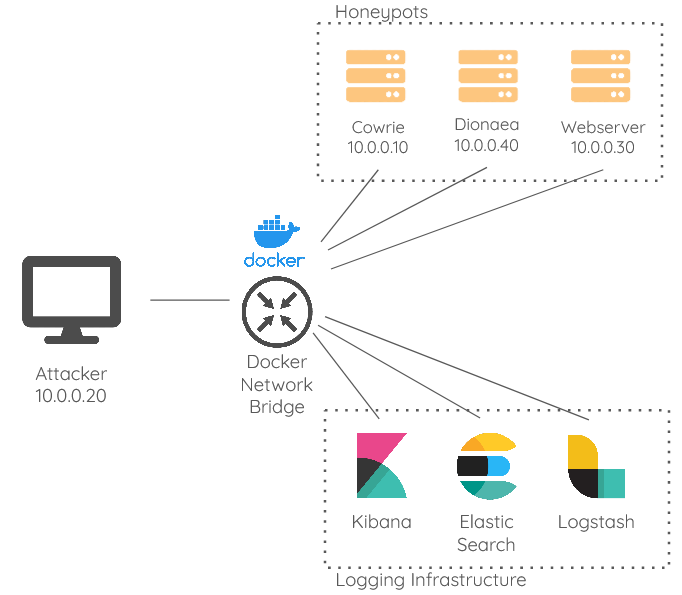
\includegraphics[scale=0.25]{topology}
\end{center}
The docker-compose.yaml file containing the definition for the containers can be found in the netsec-honeypot-lab folder on the desktop or in our Github public repository: 

\url{https://github.com/Marcy-P/netsec-honeypot-lab}

\noindent The repository README also contains additional info for accessing the containers and the references to some Docker images we used.

\section*{Starting up the lab}
To start the laboratory login into the VM with the credentials: username: \textit{netsec} and password: \textit{password}. Then open a terminal in the folder \textbackslash netsec-honeypot-lab on the desktop and type the following command:

\begin{lstlisting}[language=bash]
$ ./start.sh
\end{lstlisting}

\section*{Shutting down the lab}
To shut down the docker-compose network type:

\begin{lstlisting}[language=bash]
$ docker-compose down
\end{lstlisting}

\noindent To also clean the persistent data present in Elasticsearch type:

\begin{lstlisting}[language=bash]
$ docker-compose down -v
\end{lstlisting}

\newpage

\chapter{What is a honeypot?}
\label{cha:intro}

"A honeypot is a network-attached system set up as a decoy to lure cyber attackers and detect, deflect and study hacking attempts to gain unauthorized access to information systems"\cite{techtarget}. So it is a system that is unprotected and serves no business purpose but sits in the network waiting to be contacted. Every interaction with a honeypot is suspicious because no legitimate user should utilize it.

\chapter{Characteristics of a honeypot}
\label{cha:characteristics}

Honeypots have four main characteristics; they have to be: \textbf{Deceptive} , \textbf{Discoverable}, \textbf{Interactive}, \textbf{Monitored} \cite{sanders2020intrusion}.

\section{Deception}

Deception can be defined as an advantageous distortion of an adversary's perceptions of reality. Honeypots heavily use this concept as a tool because they appear as real systems, but they do not serve any functional purpose for a business.

There are various frameworks that try to classify various deception strategies, and we considered the taxonomy proposed by Bell and Whaley \cite{Whaley}. According to this model deception consists in two main parts: hiding the real (dissimulation) and showing the false (simulation).

Honeypots are meant to be reachable, so you do not hide it entirely, but you often have to hide specific features of them to make them less suspicious.
The techniques to hide the real are:
\begin{itemize}
\itemsep0em 
\item \textbf{Masking}: hide the  real by making relevant objects be undetectable or blend into the background;
\item \textbf{Repackaging}: hide the  real by making it appear like it is something different;
\item \textbf{Dazzling}: hide the real by altering an object to confuse the adversary;
\end{itemize}

The techniques to show the false are:
\begin{itemize}
\itemsep0em 
\item \textbf{Mimicking}: show the false by using characteristics present in the actual real object;
\item \textbf{Inventing}: show the false by giving the perception that a relevant object exist while it does not; 
\item \textbf{Decoying}: show the false by misdirecting and attracting the attacker attention away from real objects.
\end{itemize}
Note that not every honeypot has to strictly follow these techniques. It is just a theoretical framework that you may want to use when creating and deploying a honeypot. 
A more in depth analysis of the usage of deception for cyber defense can be found in the following paper "Deception used for Cyber Defense of  Control Systems" \cite{deception_defense}.

\section{Discoverability}
Honeypots are not meant to be accessed by legitimate users but just the attacker. So when designing your honeypot you have to consider the point of view of the attacker.
In particular, you can ask yourself the following questions:
\begin{itemize}
\item Where is the attacker more likely to enter your network?
	\begin{itemize}
	\item User workstations
	\item Vulnerable services exposed to the internet
	\item Stolen VPN credentials
	\end{itemize}
\item What tool will they use to discover your asset?
\item What assets will they be interested in?
\end{itemize}

To increase discoverability, you might also place \textbf{breadcrumbs} in systems that might be compromised. They are data that will lead the attacker to your honeypot while the attacker is gathering information needed to do lateral movement in the network. An example of breadcrumbs is a clear text document containing an URL or IP of a honeypot and some credential or SSH private keys.

\section{Interactivity}

Technically a single attacker interaction is enough to produce an alert. But is better if the honeypot responds back to the attacker for two main reasons:
\begin{itemize}
\item Each interaction that attacker does with the honeypot could provide you important information. For example, if they stole some credential, you may be able to know the account that was compromised. You may be able to find out what tool they use to enter  your network
\item Make the attacker waste time. Every second that the attacker spends interacting with the honeypot is a second you can invest into finding out which systems were compromised and isolate the attacker
\end{itemize}



\section{Monitoring}

Finally, honeypots have to be monitored. This means that every notable interaction with a honeypot must generate an event or alert. This alert generally gets fed to a central SIAM that is accessible to the network administrator or security team.

To manage all the event generated in an environment with multiple honeypots, you have to build a \textbf{logging and monitoring infrastructure} that stores the logs and alerts the analyst of the presence of an attack. The process of shipping logs from the honeypot to the monitoring server usually happens in four phases:
\begin{enumerate}
\item \textbf{Source}: the data are generated from the honeypot. Note that each honeypots produce logs in their own format. You need to be aware of such format because often it is not compatible with the Logging and Monitoring Server.
\item \textbf{Egress}: the data are transmitted to a central location. There has to be a sender capable of reading the logs and sending them to another location. In this phase you also can do some filtering  if some of the information provided in the logs are not needed or conversion to other formats. 
NB: Since you are transferring data over the network you have to consider all the CIA properties because the logs are sensitive data. If you do not encrypt data, you are vulnerable to various attacks that we already see in other laboratories. Can you guess some of them? ARP cache poisoning and MITM. If the attacker can intercept the logs, it can know that a system is a honeypot without never interacting with it!

\item	\textbf{Ingress}: the data are received. There should be a component that receives logs and parses them in a format compatible with the destination. In this phase it is also important to do additional filtering because  some honeypots are very noisy. You may want to filter out interaction that are not important [e.g., not log whey they interact for the first time with the honeypot but just when they authenticate] or interaction from component of the network that may interact with the honeypot (e.g., scanners)
\item \textbf{Destination}: The data are stored in the destination inside a database.  You also can implement a dashboard to see them. This component must be protected because like already said these logs are sensitive data. You may also want a system to backup important logs.
\end{enumerate}

Another mechanism that you can implement in parallel to the logging infrastructure is a monitoring infrastructure. You do not want to miss an attack because a honeypot was down because of a crash. This infrastructure allows to keep track of the status of each honeypot and alert you when a honeypot goes down.

\chapter{Honeypots classification}

Honeypots can be classified on the basis of different characteristics. The two main classifications are based on level of interaction and on the goal.

\section{Based on level of interaction}

Honeypots are classified by their degree of interaction with the communication destination (attacker) as a low interaction, medium interaction or  high interaction type. However, this does not mean that one type is better than the others. These terms are used in different ways depending on implementation, usage and purpose.

\begin{itemize}
\item \textit{Low interaction}: low interaction honeypots capture the information about the predetermined activities of attackers, and limit these activities by using emulation software. They exclusively utilize emulation software and its services, hence the quality of these honeypots is decided by the quality of emulation software. They are easier to maintain and deploy, and are also more secure compared to high interaction honeypots, because the attacker’s action is limited in the emulated area of the computer. Nonetheless, because it does not imitate the actual OS or application completely, the attacker may recognise this machine as a honeypot. 

\item \textit{High interaction}: high interaction honeypots allow the attackers interacting with real systems and do not assume anything about the possible behavior of the attacker. They help the administrator to investigate the complete activities of the attackers, utilizing the operating systems (e.g. Linux) and applications (e.g. FTP) without using the emulation software (e.g. Dionaea) to record the activities of attackers. In most cases attackers are unable to recognize the honeypot because it behaves similarly to the actual target host. However these systems require more resources and are difficult to set up and maintain; also the possibility of infection from the malware or hacking by the attacker is higher than for the low interaction type honeypot. Therefore, the system should be monitored properly, and it is necessary to be prepared to restore the system to the state before the infection of malware.

\item \textit{Medium interaction}: medium-interaction honeypots are a combination of low-interaction and high-interaction honeypots, capable of emulating full services or specific vulnerabilities. Similar to low-interaction honeypots, their primary purpose is detection and are installed as an application on the host operating system with only the emulated services being presented to the public. The key feature of a medium-interaction honeypot is application layer virtualization. They do not aim at simulating a totally operational system environment, nor do they implement all details of an application protocol. They provide sufficient responses that known exploits waiting on certain ports are going to be tricked into sending their payload. Once this payload has been received, the shellcode can be extracted and analyzed. After that, the honeypot emulates the actions that the shellcode would take to download the malware.
 
\end{itemize}

\section{Based on the goal}

\begin{itemize}
\item \textit{Research honeypots}: these are deployed by various security researchers to assess cyber threats, study the real motivation behind the attacks and capture various zero-day exploits. They help in gathering information about attacks and what kind of hacking (attacking) techniques are being used by the attackers. Various logging tools are used to log each and every activity happening on the honeypot, which can really help researchers to study the various advanced methodologies used by an attacker. They mainly consist of high interaction honeypots, in fact they are complex to deploy and maintain.


\item \textit{Production honeypots}: these are deployed by organizations to mitigate threats and protect themselves from various attacks. They require less resources and can be easily deployed. Production honeypots are often placed near security assets, in order to alert defenders of an attack; they are cheap and usually belong to the low interaction type. Use of low interaction type includes port scan identification, generation of attack signatures, trend analysis and malware collection. On the other hand, this is also a disadvantage, indeed it is not possible to watch how an attacker interacts with the operating system as all the services are emulated.


\end{itemize}

\chapter{Advantages of honeypots}
Honeypots present certain advantages over other defense systems, which is why they should be considered in the development of a well-secured network.

Firstly they consume few resources, especially if compared to traditional IDSs. While an IDS may have to handle gigabytes of data per second, a honeypot has just to handle the activities directed to itself. But it’s important to remember that honeypots are not a substitute for IDS, because usually honeypots are more a reactive control, whereas IDSs act more as preventive controls. Also IDSs deal with known threats (but not only) while honeypots deal with unknown one.

A second advantage is the fact that they are simple and cheap  to maintain. Especially for those belonging to the low interaction type, you can prepare a script that can deploy hundreds of honeypots in your network.

As a third advantage they produce a small number of logs with few false positives, because there is no reason for legitimate users to access the honeypot. So you do not need a whole team of security experts that have to keep checking alerts.

\chapter{Cowrie}

\section{What is Cowrie?}

Cowrie is an open-source medium interaction SSH, and Telnet honeypot designed to log brute force attacks and the shell interaction performed by the attacker \cite{whatcowrie}.
It can run in two modes:
\begin{itemize}
\itemsep0em 
\item In Medium interaction mode (shell) it emulates a UNIX system. To do so it provides:
	\begin{itemize}
	\itemsep0em 
	\item An authentication mechanism via SSH
	\item A  post authentication shell
	\item The ability to create fake file system with files that attacker can cat
	\item A mechanism to save files downloaded inside the shell with wget, curl or uploaded with SFTP and scp
	\end{itemize}
\item In High interaction mode (proxy) it functions as an SSH and telnet proxy to observe attacker behaviour to another system. To use this mode you have to provide a real secure backend environment where the attacker can execute any Unix command.
\end{itemize}

\noindent In this lab we will just focus on the Medium interaction mode because is the most popular one and can be used easily inside a virtual machine.


\section{Start-up Cowrie}
To enter in the Cowrie Docker instance open a terminal in the \textit{netsec-honeypot-lab} folder and type:
\begin{lstlisting}[language=bash]
$  ./startup/cowrie.sh
\end{lstlisting}
Cowrie is already installed and you can start it by typing:
\begin{lstlisting}[language=bash]
$ cowrie start
\end{lstlisting}
You will find the logs in the folder \texttt{var/log/cowrie/cowrie.log}. To print them as they get generated execute the following command:
\begin{lstlisting}[language=bash]
$ tail -f var/log/cowrie/cowrie.log
\end{lstlisting}

\section{Brief exercise - The attacker point of view [4-5 minutes]}
Enter in the attacker machine by typing in another terminal:
\begin{lstlisting}[language=bash]
$ ./startup/attacker.sh
\end{lstlisting}
As the attacker, you successfully installed nmap on the compromised machine and identified a host with the IP 10.0.0.10 (Cowrie IP address). Try to execute a probe scan to see what services run on that host. You can do it with the command:
\begin{lstlisting}[language=bash]
$ nmap -sV 10.0.0.10
\end{lstlisting}
You should see that with the Cowrie default configuration the (fake) SSH service run on port 2222.
Now you should try to connect using common credential for example username: \textit{root} and password: \textit{password}. To do that type the command:
\begin{lstlisting}[language=bash]
$ ssh root@10.0.0.10 -p2222
\end{lstlisting}
Once you are logged in inside the honeypot, play a bit in it and list some strange behaviours you encountered that suggest you that the system is a honeypot.
Things to keep in mind:
\begin{enumerate}
\itemsep0em 
\item With the default configuration there is a time-out that will log you out every two minutes
\item While inside the honeypot don't worry about breaking things.
\item If you get stuck for some reason type in the cowrie terminal: \$ cowrie stop and then start it again.
\end{enumerate}

\section{Brief exercise - Solution}
Here a list of behaviour you may have encountered:
\begin{itemize}
\itemsep0em 
\item If you type the command:
	\begin{lstlisting}[language=bash]
$ uname -v
	\end{lstlisting}
	You get that the system is a Debian Linux distribution. So you may want to try to install some software. For example by typing:
	\begin{lstlisting}[language=bash]
$ apt-get install ftp 
	\end{lstlisting}
	But after the installation screen every time you try to execute the newly installed command you will get the error SEGMENTATION FAULT.
\item When you try to \texttt{cat} some files they seem to exist but you will get the error "\textit{No such file or directory}"
\item You cannot kill processes
\item You are able to downloads  file with wget but when you check their size with the command ls -al you see them as 0 Byte files
\item If you delete all the files in the root folder nothing breaks. And if you re-login into the honeypot all the file will return.
\end{itemize}

\section{A consideration about the previous exercise}
Some may think that is not that hard to figure out that the system is a honeypot, but you have to keep in mind that when the attacker is inside the honeypot we already logged every character he typed.
You can actually replay each session of interaction with the command:
\begin{lstlisting}[language=bash]
$ bin/playlog var/lib/cowrie/tty/[session_log_ID]
\end{lstlisting}
And also check the files that the attacker downloaded by checking the following folder:

\begin{lstlisting}[language=bash]
$ ls var/lib/cowrie/downloads/
\end{lstlisting}

\section{Customizing Cowrie}
The honeypot with the default configuration is almost empty, but the goal is to make the attacker believe that it is a legitimate system. In this way you can increase its interaction with the system and gather intel about what is seeking or what tool it uses. To make Cowrie resemble a legitimate system you have to start by modifying the cowrie config files.

The first thing to do is to copy the default configuration file \texttt{cowrie.cfg.dist} in a file named \texttt{cowrie.cfg}, Cowrie will give priority to this file if it exist:
\begin{lstlisting}[language=bash]
$ cd etc
$ cp cowrie.cfg.dist cowrie.cfg
\end{lstlisting}
Now you can access the file with a text editor (e.g. vim or nano) and edit the following sections:
\begin{itemize}
\item Scroll down a bit and change the \texttt{hostname}. You might want to mimic similar server name existing in the network range of the honeypot. Or you can also stand out with something original.
\item Search for timeout to change the interaction and authentication timeouts to a new value
\item Search for \texttt{listen\_endpoints} in the \texttt{[shell]} section (second match of the search) and modify the port from 2222 to 22
\end{itemize}

\noindent NB: for every modification you want to apply remember to restart Cowrie with the command:

\begin{lstlisting}[language=bash]
$ cowrie restart
\end{lstlisting}

\subsection{Modifying the login credentials}
\label{sub:login}
Another fundamental part to customize are the credentials that the attacker can use to SSH into the honeypot. To achieve this copy the file \texttt{userdb.example} to \texttt{userdb.txt}:
\begin{lstlisting}[language=bash]
$ cd etc
$ cp userdb.example userdb.txt
\end{lstlisting}
Inside this file you will find an explanation of the syntax to use.
Try to use generic credentials that can be easily guessed but without raising suspicion.


\subsection{Modifying the process list}
Cowrie allow you to create a list of fake processes that will be printed with the command \texttt{ps}. To do that modify the JSON file at the following path: \texttt{share/cowrie/cmdoutput.json}. The syntax is self explanatory. When you edit it try to remove processes that are not likely to appear in your system and add processes that are running on a real systems


\subsection{Modifying the file system}
Cowrie provide an emulated file system so when an attacker login it will get its own personal copy of this filesystem that will be deleted when they log off. This file system is implemented into two components:
\begin{itemize}
\itemsep0em 
\item \textbf{pickle file}: contains metadata for the files (their name, size, permission, directory, …)
\item \textbf{honeyfs directory}: contains the file contents
\end{itemize}

\noindent NB: to be visible (\texttt{ls}) a file must be in the pickle file, and to be also accessible (\texttt{cat}) it needs to be in the honeyfs directory.

You can find the \texttt{honeyfs} directory in the cowrie installation folder. An interesting file you can modify is \texttt{motd} that contain the SSH post login banner.
\begin{lstlisting}[language=bash]
$ cd honeyfs
$ vim etc/motd
\end{lstlisting}

If you created a new user credentials in the section \ref{sub:login} remember to create also the home directory for that user.
Also, for the next section create a file \texttt{/bin/nmap}.

Finally you can generate the pickle file automatically by typing:
\begin{lstlisting}[language=bash]
$ rm ./share/cowrie/fs.pickle
$ ./bin/createfs -l honeyfs -d 5 -o ./share/cowrie/fs.pickle
\end{lstlisting}
The flag \texttt{-l} is used to specify the location of the honeyfs folder, the flag \texttt{-d} sets the depth of the file system you want to include. Finally the flag \texttt{-o} sets the location of the pickle file you are creating. Cowrie will search for the pickle file in the \texttt{./share/cowrie/} directory.



\subsection{Adding new commands}

To add a new command add a file in the folder \texttt{share/cowrie/txtcmds/bin} containing a static output for that command. Previously we created the binary file for nmap so now you can try to create an output for nmap.
\begin{lstlisting}[language=bash]
$ vim share/cowrie/txtcmds/bin/nmap
\end{lstlisting}
Now when executing the command \texttt{nmap} the attacker will receive the static output you specified.

\chapter{Dionaea}

\section{Dionaea Architecture}

\subsection{Introduction}

As described in \cite{dionaea}, Dionaea is the successor of the Nepenthes system and belongs to the low interaction type. The main goal of Dionaea is to trap malwares exploiting vulnerabilities exposed by services offered to a network, the ultimate goal is gaining a copy of the malwares.

Dionaea, like any software, is likely to contain bugs that may be exploited. In order to reduce the effect, Dionaea runs in a limited environment with no administrative access. It emulates services such as FTP, HTTP, MSSQL (Microsoft SQL server), MySQL, SMB, TFTP, SIP and others; these services emulate a vulnerable server running Windows OS. SMB is the most vulnerable service running in Dionaea, which utilizes well-known port 445.

In addition, this honeypot has the following features:
\begin{enumerate}
\itemsep0em 
\item It is composed of a modular architecture, embedding Python as its scripting language in order to emulate protocols;
\item It supports IPv6 and TLS (Transport Layer Security);
\item It can obtain a detailed analysis of captured malwares, by sending them automatically to the VirusTotal platform.
\end{enumerate}

\subsection{Exploitation}

Dionaea has to detect and evaluate the payload to be able to gain a copy of the malware. In order to do so, Dionaea uses libemu. Given certain circumstances, libemu can detect shellcode, measure the shellcode, and if required even execute the shellcode.

Shellcode measurement/profiling is realized by executing the shellcode in the libemu virtual machine and recording API calls and arguments. In most of the cases shellcode profiling is sufficient, since the recorded API calls and arguments reveal enough information to get an idea of the attackers intentions. For multi-stage shellcode, where the first exploitation stage of the shellcode would retrieve a second shellcode from the attacker, profiling is not sufficient, as we don’t know what will happen from the second stage of the shellcode. In this case we need to make use of shellcode execution: this is basically the same as shellcode profiling, the only difference is that api calls are not recorded, and also the shellcode is allowed to perform certain actions.

After the shellcode profiling has been done, Dionaea has to guess the intention, and act upon it.

\subsection{Logging}

Dionaea offers a logging system which logs all the activities in a clear text file, which can be used for analysis and attack prediction. However, this type of logging to a text file is very chatty, and you do not want to use it unless for debugging or development purposes.

In addition to that, Dionaea uses some internal communication system which is called incidents. Incidents, containing information about the origin and properties of an “attack”, are passed using incident handlers (ihandlers). An ihandler can register a path for incidents he wants to get informed about, and  the paths are matched in a glob like fashion. Therefore logging information using an ihandler is superior to text logging, because you get the information you are looking for, and can write it to a format you choose yourself; in other words it’s a more scalable solution.

The most useful ihandler is the \texttt{log\_sqlite}, which writes interesting incidents to a sqlite database. One of the benefits of this logging is the ability to cluster incidents based on the initial attack when retrieving the data from the database; another interesting one is the \texttt{log\_json} ihandler, which permits to save the logs in JSON format. JSON logs can then be used, for example, to configure Dionaea to work with ELK stack.

Dionaea can also dump a connection as bi-directional stream. These bi-directional streams are pretty useful when debugging, as they allow replaying an attack on ip-level. You can specify the directory where these are stored in the configuration file. Default is storing them in the directory \texttt{/opt/dionaea/var/lib/dionaea/bistreams}.

\subsection{Analysis}

After Dionaea has obtained a copy of a malware, it can either store the binaries locally or submit the file to some external tools or services (e.g. CWSandbox, Norman Sandbox, VirusTotal, etc.) for further analysis.

\section{Let's see in practice}

\subsection{Access to Dionaea}


To enter in the Dionaea Docker instance open a terminal in the netsec-honeypot-lab folder and type:

\begin{lstlisting}[language=bash]
$ ./startup/dionaea.sh
\end{lstlisting}

\noindent At this point you are in the Ubuntu file system. In order to enter in the directory of the honeypot, type:
\begin{lstlisting}[language=bash]
$ cd opt/dionaea
\end{lstlisting}

\noindent Dionaea has already started automatically when the docker container was created. Otherwise, if the machine has not already started, it is possible to start it using the command:
\begin{lstlisting}[language=bash]
$ /opt/dionaea/bin/dionaea
\end{lstlisting}
The startup options can be displayed adding the \texttt{-h} flag. Another interesting one is the \texttt{--config=FILE} option, with which you can use FILE as the configuration file; the default behaviour is using the file \texttt{/opt/dionaea/etc/dionaea/dionaea.cfg}.

\subsection{Directory Structure}

In the Dionaea directory you can find different folders: those of greatest interest are the \texttt{etc} and \texttt{var} folders. In the first you can find the configuration file, the services and ihandlers available, and the services and ihandlers enabled, whereas the second folder contains the log files, the binaries downloaded by Dionaea, and also the sqlite database. In particular the text log file is at the path \texttt{/opt/dionaea/var/log/dionaea/dionaea.log}.

You can see that there is also a python script named \texttt{readlogsqltree.py}: this is a python3 script which queries the Dionaea sqlite database for attacks, and prints out all related information for every attack; this tool provides information about the exploited vulnerability, the time, the attacker, information about the shellcode, and the file offered for download (if any). To create such report for your own honeypots activities for the last 24 hours run:
\begin{lstlisting}[language=bash]
$ python3 readlogsqltree.py -t $(date '+%s')-24*3600 
/opt/dionaea/var/lib/dionaea/dionaea.sqlite
\end{lstlisting}
At the moment no connections are printed, because there are not any yet.

\subsection{Port scan}

As a first task let’s perform a port scan on the honeypot. This will show us the services running in the honeypot, and it will also reveal a strange result. In the same way done for Cowrie, enter in the attacker machine and run the command:
\begin{lstlisting}[language=bash]
$ nmap -sV 10.0.0.40 -Pn
\end{lstlisting}
It will take about 2 minutes.

As you can see there are a lot of services running on the machine, and in particular the services running on port 445 and 1433, which are respectively the SMB and the MSSQL, are detected as Dionaea honeypot services. This happens because nmap recognises them from the responses received, which are the default responses of Dionaea. Having said that, if in the implementation of Dionaea these responses are changed, nmap will no longer be able to detect them.

Now, if you go back to Dionaea and execute again the \texttt{readlogsqltree.py} script, you will see that many connections are reported: in fact the port scan creates a lot of traffic in order to find running services, and the honeypot has recorded all of it.

\subsection{SIP OPTIONS scan}

If you paid attention to the port scan, you should have seen that there is the SIP service open on port 5060/tcp, so as a second step let’s launch a SIP OPTIONS scanning. For the next tasks, in order to simulate attacks, we will use the Metasploit Framework. Inside the attacker’s machine, type:
\begin{lstlisting}[language=bash]
$ ./msfconsole
\end{lstlisting}
to run the Metasploit console.

When Metasploit is ready, use the command \texttt{\$ search sip options\_tcp} to search the right module; after this use the command \texttt{\$ use 0} to use the module found. At this point you have to set the target host: to do this type \texttt{\$ set rhost 10.0.0.40}. Finally, run \texttt{\$ exploit} to launch the scan.

Now go back to Dionaea and execute the python script another time. You should see that the last reported connection is a SipSession tcp connection. In this case the attack does not trigger any vulnerability, because it is only a SIP OPTIONS scan. This type of scanning is executed to spot VoIP devices and determine their capabilities. It might be a reconnaissance step of a multi-stage attack. These scans are used to identify targets and the next stage will likely target only those devices which responded during scanning. \cite{ENISA}

\subsection{SMB exploitation}

The next task is to try to exploit a vulnerability on the SMB protocol on port 445. As already said, this is the main protocol offered by Dionaea. SMB has a decent history of remote exploitable bugs, and is a very popular target for worms. The vulnerability that will be attempted to exploit is that detailed in Microsoft Bulletin MS10-06; it is a vulnerability in the Print Spooler service. The vulnerability could allow remote code execution if an attacker sends a specially crafted print request to a vulnerable system that has a print spooler interface exposed over RPC.

Inside the Metasploit console, use the command \texttt{\$ search ms10-061} to search the right module; after this use the command \texttt{\$ use 0} to use the module found. At this point you have to set the printer share name to use on the target host: to do this type \texttt{\$ set pname XPSPrinter}. After this step you have to set the target host: to do this type \texttt{\$ set rhost 10.0.0.40}. Finally, run \texttt{\$ exploit} to launch the exploit.

You can see the exploit completed, but no remote code execution session was created; this happens because Dionaea is a low interaction honeypot. However, if you go back to Dionaea and run the python script, you can see that there has been a connection from the attacker on the smb protocol; also you can see that, under the "download" section, it is reported that something has been downloaded (together with the download URL). To check what has been downloaded, enter in the binaries folder, typing:
\begin{lstlisting}[language=bash]
$ cd /opt/dionaea/var/lib/dionaea/binaries
\end{lstlisting}

\noindent Here you can find two files: one is the MD5 hash value of the corresponding malware, calculated by Dionaea. This MD5 hash value is used for analysis purposes: you can either submit the hash value to VirusTotal or you can submit it to any antivirus software. You can consider this hash value as a feature of a malware \cite{malware_capturing}. The other downloaded file is a tmp file.


\subsection{MSSQL server login}

Another interesting task that you can try to perform is to log into the Microsoft SQL server, which runs on port 1433. To do this, you will again use Metasploit. Inside the Metasploit console, run the command \texttt{\$ search mssql\_login} to search the right module; after this run the command \texttt{\$ use 0} to use the module found. There is a default username already set, which is ‘\texttt{sa}’: this is the administrative username on the Microsoft SQL server. At this point you have to set the password. You can choose whatever you want, indeed the login will be always successful and the task is only performed in order to see the result on the honeypot. So, for example, use the command \texttt{\$ set password pass} to set the password as \texttt{pass}. Next you have to set the target host: in order to do this run \texttt{\$ set rhost 10.0.0.40} as in the previous tasks. Finally, run \texttt{\$ exploit} to launch the exploit. The result is that you logged in successfully.

Now return to Dionaea and run the python script again. You can see the last connection, which was on the mssql service, and also the username and the password used for the login. In this way, in a real scenario, it is possible to observe which are the most popular names used by hackers, and finding a way to substitute them with unknown ones will elevate the system’s security \cite{malicious_access}.

The same approach of login could be used for the FTP or MySQL servers.


\subsection{VirusTotal analysis}
If you want to enable Virustotal to analyse the malwares you capture, you first need a Virustotal API key. To obtain it, you have to go to the website \url{https://www.virustotal.com/} and sign up; in this way you will automatically obtain a key. Once you have the API key, you have to go to the folder \texttt{/opt/dionaea/etc/dionaea/ihandlers-available} and modify the ihandler file named \texttt{virustotal.yaml}; here you have to paste your API key in the indicated place. In this case there is already a pasted key, which is the key utilized by us. After this, save and exit. Next change the directory to \texttt{/opt/dionaea/etc/dionaea/ihandlers-enabled}. Now, you need to create a symbolic link here (which has already been created)  to the edited \texttt{virustotal.yaml} file typing:

\begin{lstlisting}[language=bash]
$ ln -s ../ihandlers-available/virustotal.yaml virustotal.yaml
\end{lstlisting}

\noindent After following this procedure, in theory your new captured malware should now be identified, and you should be able to look at the analysis running the python script used for the previous tasks. In practice however, there is actually a bug in the current version of Dionaea for which the feature does not work (but this bug will certainly be fixed soon).

Also, in the directory \texttt{/opt/dionaea/var/lib/dionaea} there is a sqlite database named  \linebreak \texttt{vtcache.sqlite}. This is used to cache the results of the performed analyzes.



\chapter{Honeyfiles}

A honeyfile is an intrusion detection mechanism based on deception. This mechanism works by creating a bait file that when accessed set off an alarm or log the access to the document. In this way you can detect unauthorized access to a computer. This is a very simple technique, but it is also very effective. Usually, in many organizations important information gets stored in office documents. So, when an attacker compromises a machine, he often checks for valuable documents.

When “setting up” a honeyfile you have to think about what the attacker is interested in. Usually they search for four types of files \cite{deceptive_files}:
\begin{enumerate}
\itemsep0em 
\item Information for accessing other systems (e.g., passwords, network details) or security documentation
\item File containing important information's like intellectual property, customer lists, product design.
\item File containing personal information that could be  used to harm reputation or allow further compromise of the system
\item Log files that can contain evidence of attacks.
\end{enumerate}

Then you have to think what the attacker will see, so:
\begin{itemize}
\itemsep0em
\item You must place the file in a way that can be easily found. But if it is a system used by legitimate users that are unaware of the honeypot, you should place it in a way that is unlikely to be accidentally opened.
\item Is very effective when the file stands out from other files. You can achieve this in various ways:
	\begin{itemize}
	\itemsep0em
	\item FILE NAME IN CAPS
	\item Usage of a document type different from the other documents around it
	\item Setting a unique or odd file size (e.g., a 23 MB word document between 15 kB documents)
	\end{itemize}
\end{itemize}

\noindent NB: Do not exaggerate by placing to many honeyfiles, because it will also increase the chance of triggering false positives by legitimate users. And also do not try to hard with the naming conventions otherwise the attacker will become suspicious.

\section{Honeydoc}
A honeydoc is a  particular type of honeyfile. In particular is an office document that contains a token used for tracking purpose (called web bug or web beacon). This token  references a resource from an external URL. In this way when the document is opened, the external resource will be requested and the server serving this resource will log the interaction. In the next exercise we will hide this web bug by shrinking it in a 1x1  pixel image.

\section{Create a LibreOffice honeydoc}

For this laboratory exercise there is already a Nginx server running that serve an image that you can use as web bug. The page is accessible by opening Firefox on the virtual machine and opening the page at the URL \texttt{localhost:8080}.
It is also possible to access to the Nginx instance to see its logs. Just open a terminal and execute the commands:
\begin{lstlisting}[language=bash]
$ docker exec -it honeydocserver /bin/bash
$ tail -f /var/log/nginx/access.log 
\end{lstlisting}

Now you can create the honeydoc. First open LibreOffice and create a new document. Then follow these steps:
\begin{enumerate}
\itemsep0em
\item Create a footer by clicking at the bottom of the page. By placing the web bug there is harder that is accidentally found or  deleted
\item Click on the Insert tab. Then insert an image. Now select just a temporary image  and then select the box "Insert as a link".
\item LibreOffice will ask if you really want to include a link. You have choose "Keep link"
\item Now right click on the image. And click on properties.
\item In the first tab resize the image as small as possible (0.2")
\item In the "option" tab check the protect content, position and size boxes.
\item In the "image" tab modify the field "File Name" to reference the remote image present on the Nginx server and click OK. After these step the image should be hard to spot. To be still visible we choose a black image but by using a white or transparent image it will be very difficult to detect.
\item Add some content to the document and save it with a relevant name (e.g. PASSWORDS.txt) 
\end{enumerate}

Now, every time we open the document, Office will attempt to load the image from the URL, thus generating requests to our web server that will log the interaction.


\section{Another way to create honeytokens}
An easy way to generate honeytoken without repeating the above procedure is provided by Thinkst with their service called Canary Tokens. You can access it by going to the website \url{https://canarytokens.org}. You will need to just specify the type of token, an email address where to receive the alerts and a reminder note for when the token is triggered. Then you can download the honeytoken document and place it where it is needed.


\chapter{Lab monitoring infrastructure}

To implement our logging infrastructure we used the Elastic Stack (also known as ELK stack) an open-source log management system composed of four components:
\begin{enumerate}
\item \textbf{Beat}: is the component that assumes the role of the egress. More technically is a family of lightweight data shippers that can be installed in each honeypot system to send various types of information. For each information there is a specific beat agent, for example:
	\begin{itemize}
	\item \textbf{Filebeat}: it is used to send logs and files. It allows also to parse common logs format. We used this agent to send our honeypot logs to Logstash.
	\item Metricbeat: agent used to ship metric data.
	\item Winlogbeat: to ship windows event logs.
	\item Heartbeat: to ship data regarding uptime monitoring
	\end{itemize}
\item \textbf{Logstash}: assumes the role of the ingress. It receives data from the various Filebeats, parse and filter them. Then sends its output (that is in JSON format) to Elasticsearch. NB: It is very powerful because you can use it to structure unstructured data and enrich them with new information (for example geo coordinates based on the IP address inside a log).
\item \textbf{Elasticsearch}: it is the destination of the data. It receives the data from Logstash, store them  in a database and indexes them. This process allows to run queries on the data and aggregate them into useful information. 
\item \textbf{Kibana}: is a web-based dashboard that is used to visualize the data present in Elasticsearch. It allows you to create real-time histograms, pie charts and maps
\end{enumerate}

\section{Exercise - Create simple dashboards in Kibana}

Now that we have multiple honeypot running that generated multiple events we can log into Kibana so see the logs from a central location.

To do that, open Firefox and go to the URL \texttt{http://localhost:5601} and login with username: \texttt{netsec} and password: \texttt{password}.

After logging in, open the menu on the left side of the screen and click on Recently viewed -> raw logs. In this page you should be able to see all the logs received and stored in the elastic search database. You can use the search bar to filter for specific values and modify the time frame of the logs that are shown by specifying a time interval in the input on the right of the search bar.

To create a dashboard click on the menu 



\chapter{Honeypots for IoT}
The tremendous growth in the interconnection of Internet of Things (IoT) devices has also increased the possibility of data breach. Thus, there is a need to protect the connected devices or a system from disclosure or network-based attack. Recent Distributed Denial of Service (DDoS) attacks which used inadequately secured IoT devices, further highlight that existing defenses are slow to detect zero day exploits and capture attack traffic. So here’s the necessity for countermeasures and honeypots have long proven effective in capturing malware, helping to counter spam and providing early warning signals about upcoming threats \cite{review}.

Below are reported some recent IoT honeypots that have been developed in order to face this security problem.

\section{SIPHON}

SIPHON is a prototype of a scalable and reliable high interaction honeypot with the aim to learn about existing and novel attack vendors, be it human or automatic, targeting IoT devices. By constructing tunnels between public IP addresses and physical devices utilizing the entrypoint (wormhole), SIPHON enables the portrayal of physical IoT devices in a broad variety of geographic locations. The traffic data is gathered in order to be processed and analyzed further. The figure below represents the SIPHON architecture with IP cameras and a networked video recorder (NVR) linked to three different cloud servers. \cite{guarnizo2017siphon}
\begin{center}
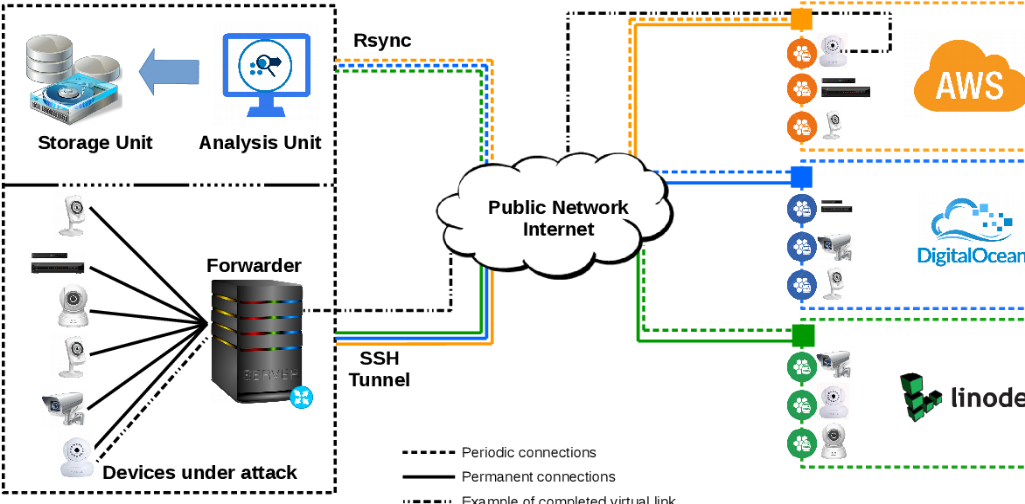
\includegraphics[scale=0.25]{SIPHON}
\end{center}

\section{HIoTPOT}

HIoTPoT functions as a camouflaged monitoring camera on the attackers, diverting them from their goals by keeping them busy in a fake environment.. It will gather any important information about the attackers. When it notices an attacker, HIoTPoT sends out notifications to all nearby IoT devices in the network, telling them not to communicate with that attacker, and so keeping the active environment secure.. HIoTPoT can act as a production honeypot as well as a research honeypot. The HIoTPOT will maintain a database for all authenticated users. Whenever a user connects to the IoT network, HIoTPOT will check that user against the database. If it finds the user in the database, then it will permit the user to enter in the real IoT environment. If it does not find the user in the database, then it will send the user to a fake IoT environment which is only an image of the real IoT environment. The intruder then believes he has gained access to the IoT infrastructure and begins interacting with IoT devices. At the same time the HIoTPOT will keep one database that will record all the intruder's communications information \cite{gandhi}.

\section{IoTPOT}

IoTPOT is a medium-interaction honeypot which emulates Telnet services of IoT devices to analyze ongoing attacks. IoTPOT has a function that automatically exeutes an active scanning of the attacking IP addresses to obtain their banner profiles. IoTPOT design is composed of a front-end low-interaction responder and back-end high-interaction virtual environment called IoTBOX which works as a malware sandbox. This IoTBOX manages various virtual environments and supports different CPU architectures \cite{IoTPOT}.
\begin{center}
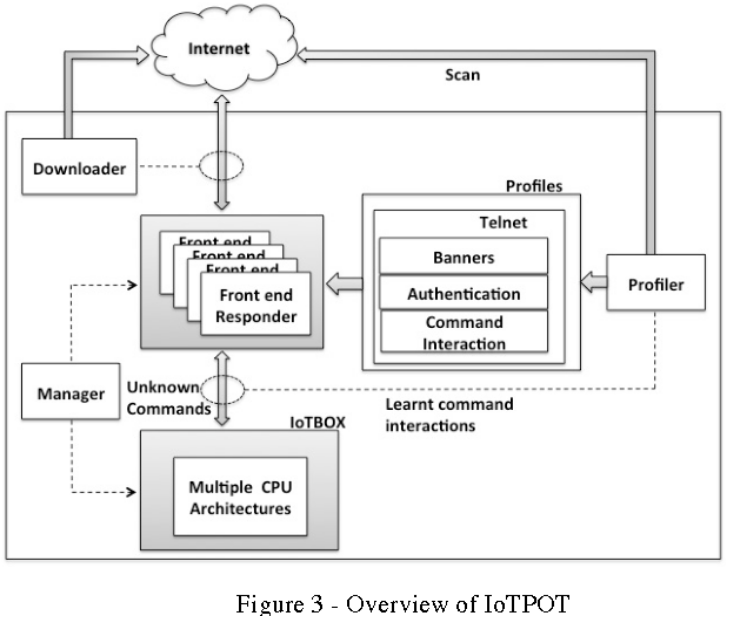
\includegraphics[scale=0.35]{iotpot}
\end{center}

\section{ThingPot}
ThingPot is a honeypot implementation of XMPP protocol (XMPP is a communication protocol that provides basic instant messaging (IM) and presence functionality) which focuses on the use case of Philips Hue (Philips Hue consists of wireless LED light bulbs and a wireless bridge). 

It can simulate an entire IoT platform rather than a single application layer communication. Additionally, the ThingPot’s source code is open to the public and is available online at Github; this includes two modules: client and server. To reduce the chances of an attacker gaining access to the real system, the ThingPot runs in an isolated simulated environment.. REST is used to build a backend API. Given its popularity, XMPP has been selected as the IoT protocol for real-time communication. The frontend is realized through a simple HTTP web service \cite{wang2018thingpot}.
\begin{center}
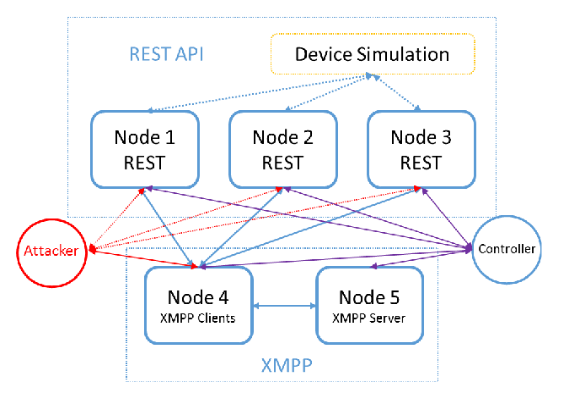
\includegraphics[scale=0.40]{thingpot}
\end{center}


\section{Honware}

As discussed in \cite{Honware}, this is the first flexible and generic framework to efficiently and effectively deploy honeypots for networked devices on the Internet to log attacker traffic and their actions. 
Honware utilises device firmware images (which are widely available for download) and a special prebuilt Linux kernel to emulate device behaviour within a virtual environment (so it doesn’t utilise real devices);
The performance of honware is comparable to real devices and is not susceptible to trivial fingerprinting based on timing attacks;
Using firmware images is cheaper and therefore more scalable.
Below is represented the honware architecture overview.
\begin{center}
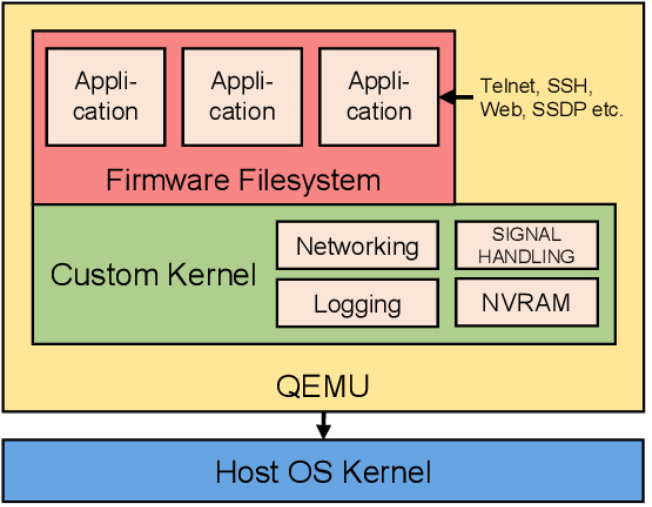
\includegraphics[scale=0.25]{honware}
\end{center}
\endgroup


% bibliografia in formato bibtex
%
% aggiunta del capitolo nell'indice
\addcontentsline{toc}{chapter}{Bibliography}
% stile con ordinamento alfabetico in funzione degli autori
\bibliographystyle{plain}
\bibliography{biblio}
\end{document}
